%\section{Описание входных данных}
Для того, чтобы провести практическое сравнение по критериям эффективности
было проведено тестирование на реальных исходных данных с помощью программного
обеспечения, описанного в предыдущем разделе. Опишем данные, на которых
проводилось тестирование.

Тестирования проводились на новейшем сформированном
множестве данных MovieLens \cite{ml-data}.
Эти исходные данные были собраны компанией MovieLens, которая
занимается исследованиями и разработками в области РС. Исходные
данные не являются синтетическими данными, а данными,
которые были заполнены реальными
пользователями. Множество данных MovieLens характеризуется следующими
показателями:
\begin{itemize}
	\item $|U| = 700$;
	\item $|I| = 9000$ --- объектами являются фильмы;
	\item $|P| = 100000$;
	\item $|Y| = 18$ --- характеристикой фильма является кинематографический
		жанр.
\end{itemize}
Список жанров-характеристик объектов:
\begin{itemize}
	\item action;
	\item adventure;
	\item animation;
	\item children's;
	\item comedy;
	\item crime;
	\item documentary;
	\item drama;
	\item fantasy;
	\item film-Noir;
	\item horror;
	\item musical;
	\item mystery;
	\item romance;
	\item sci-Fi;
	\item thriller;
	\item war;
	\item western.
\end{itemize}

Для АКМ $X = I$ и $w_U(u, x) = \rho(u,x), x \in I$.

Для задания правила вывода $\Pi_f$ была аналитически определена
функция $\delta_c$, основываясь на эвристическом предположении о том,
что между оценкой близости $\rho(u, i)$, заданной пользователем $u$
и характеристикой $y \in Y$ объекта $i$,
то есть жанром фильма, существует корреляция:
\begin{multline}
	\delta_c(i, y) = \frac{1}{|\{i: \exists \rho(u,i)\}|}
	\cdot
	|\{ i : (\rho(u, i) < \varepsilon_1) \wedge (\nu(y) = 1)\}| -\\
	|\{ i : (\rho(u, i) > \varepsilon_2) \wedge (\nu(y) = 1)\}|, \\
	\text{ где }
	\varepsilon_1 = 0,2, \varepsilon_2 = 0,6;
\end{multline}

Такое эвристическое предположение верно не для всех пользователей, так как
их вкусы могут быть неоднородными. Поэтому для некоторых пользователей функция
$\delta_c$ задана так, что
$|\rh(u, i_{\bot}) - \rho(u, i_{\bot}) \le \varepsilon_p|$,
а для некоторых --- нет.

\section{Сравнение моделей по критерию качества решений}

\subsection{Задача $topN$}

Результаты представляются графиком и таблицей для каждого пункта.
Координатой оси $X$ является идентификатор пользователя, координатой
оси $Y$ является значение оценки качества.
В качестве функции $\eit$ использовалась функция
<<точность>> (P) \ref{precision}.
Другие функции рассматривались так же, но между
функциями одного класса существует корреляция и приведение других графиков
оказывается избыточным.

На графиках представляются данные по двум методам тестирования. Для наглядности
результирующие данные были отсортированы по значениям оценки качества,
принадлежащим первому методу (в каждой паре точек, которые находятся на одной
вертикали, идентификаторы пользователей совпадают).

В таблицах представлены средние значения оценок точности по всем пользователям.


Для проведения тестов данного пункта исходные данные были
стандартно разбиты на тестовое и обучающее множество по следующему принципу:
разбиение проводилось случайно, в обучающее множество входит
80\% данных, в тестовое --- оставшиеся 20\%. В тестировании участвовало
подмножество $P^{\prime} \subset P, P^{\prime} = \{(u, i, \rho(u, i)):
\rho(u, i) = 1\}$.

\subsubsection{Влияние свойства транзитивности на ООМ при решении задачи $topN$}
В данном пункте приведем и сравним результаты решения задачи $topN$, полученные:
\begin{enumerate}
	\item  в ООМ при следующих параметрах:
		\begin{itemize}
			\item
			стандартный алгоритма решения задачи
			$topN$ (\ref{alg:topn-solve-ors}), основанный на
			правиле вывода $\Pi_O$;
			\item
			пороговое значение $\Delta_i$ равно $0,9$;
			\item
		применяемая мера сходства --- косинус угла (\ref{sim-cos})
		между контентами, которые представляются в ООМ в виде векторов.
		\end{itemize}
	\item  в ООМ при следующих параметрах:
		\begin{itemize}
			\item
			стандартный алгоритма решения задачи
			$topN$ (\ref{alg:topn-solve-ors}), основанный на
			правиле вывода $\Pi_O$;
			\item
			пороговое значение $\Delta_i$ равно $0,49$;
			\item
		применяемая мера сходства --- косинус угла (\ref{sim-cos})
		между контентами, которые представляются в ООМ в виде векторов.
		\end{itemize}
\end{enumerate}

При $\Delta_i = 0,9$ вероятность того, что $(i \rt j) \wedge (j \rt k)
\Rightarrow (i \rt k)$, выше, чем при $\Delta_i = 0,49$.
На Рис. \ref{pic:topn_trans} приведены результаты решений задачи $topN$ при
различных пороговых значениях. Черным цветом приведены результаты для
$\Delta_i = 0,9$, красным --- для $\Delta_i = 0,49$.
Видно, что при $\Delta_i = 0,9$ результаты решений эффективней, так
как большинство точек, соответствующих $\Delta_i = 0,9$ проходит ниже точек,
соответствующих $\Delta_i = 0,49$, что также подтверждается табличными данными,
представленными в таблице (\ref{tbl:topn_trans}).

Некоторые результаты при $\Delta_i = 0,9$ хуже, чем при
$\Delta_i = 0,49$. Это происходит для тех пользователей,
для которых характерно свойство неоднородности.

\begin{figure}[H]
	\caption{Влияние свойства транзитивности на ООМ при решении задачи $topN$}
	\label{pic:topn_trans}
	\begin{center}
		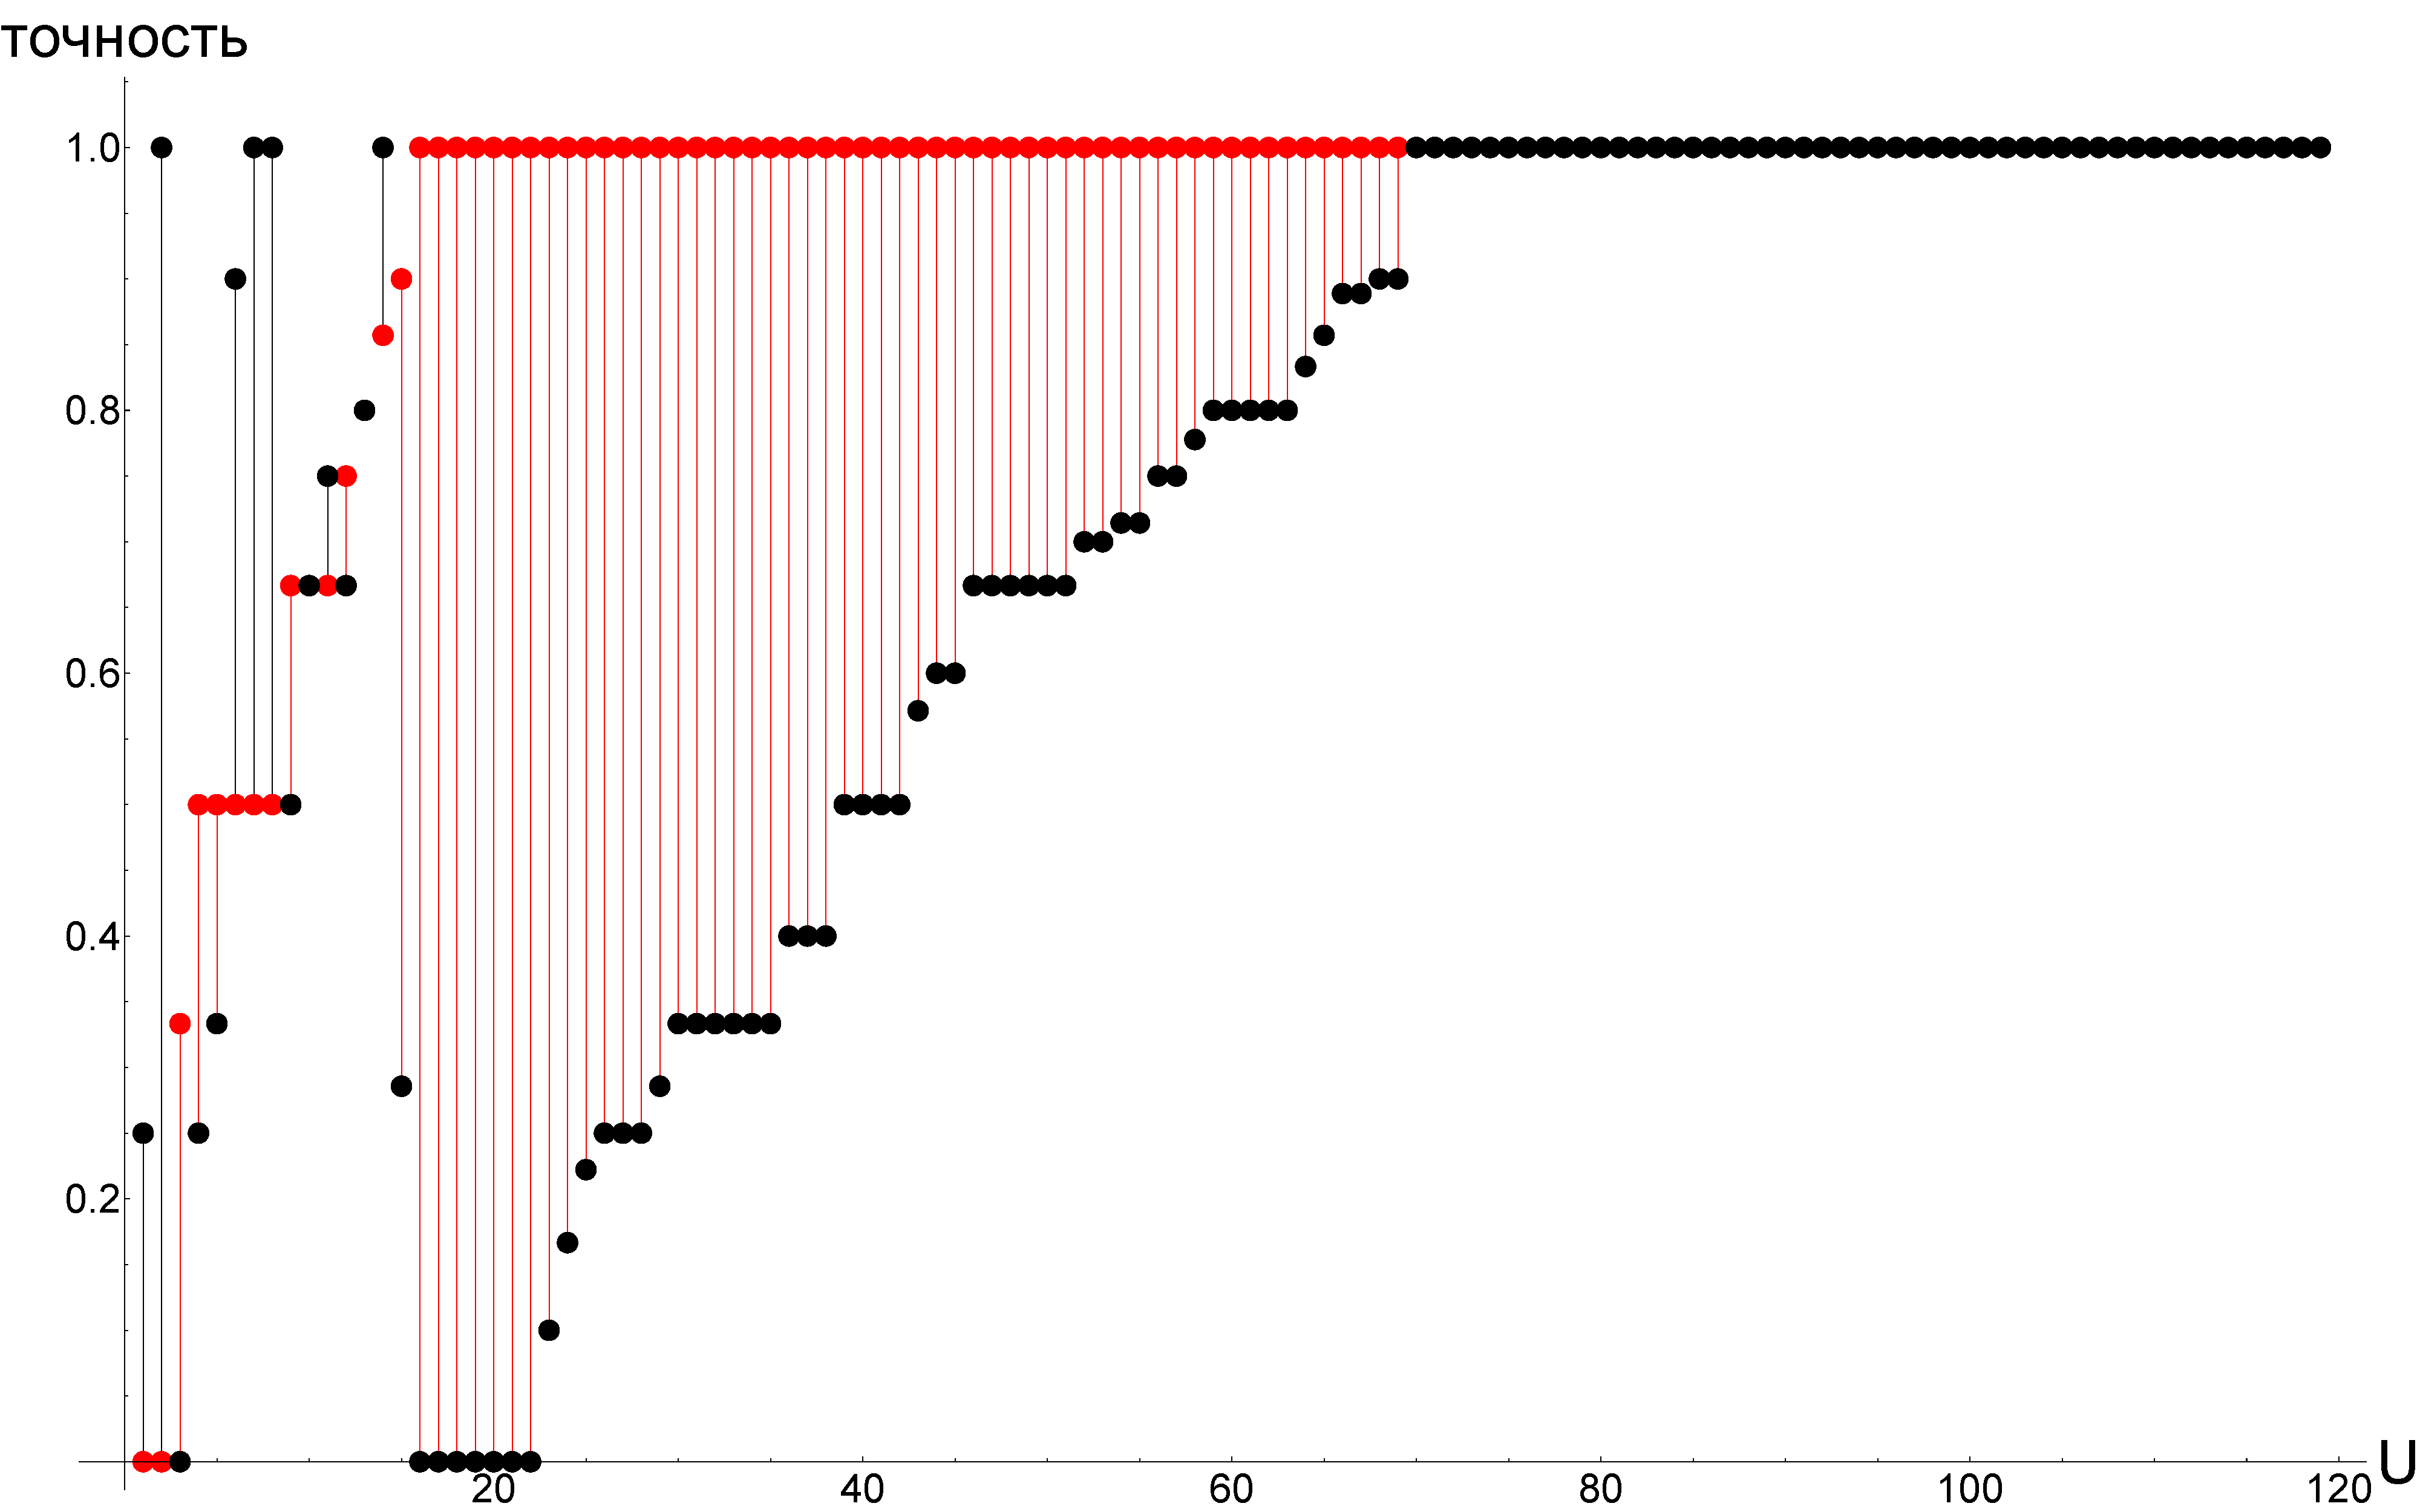
\includegraphics[width=7in,height=4in]{pics/results/transitivity.pdf}
\end{center}
\end{figure}

\begin{table}[H]
	\caption{Влияние свойства транзитивности на ООМ при решении задачи $topN$}
  \label{tbl:topn_trans}
  \begin{center}
	\begin{tabular}{|c|c|}
	  \hline
		Модель& Точность \\ \hline
		ООМ&0,925 \\ \hline
		Нечеткая&0,627 \\ \hline
	\end{tabular}
  \end{center}
\end{table}

\subsubsection{Применение правила вывода ООМ в коллаборативной и нечеткой
моделях}
В данном пункте приведем и сравним результаты решения задачи $topN$, полученные:
\begin{enumerate}
	\item  в ООМ при следующих параметрах:
		\begin{itemize}
			\item
			стандартный алгоритма решения задачи
			$topN$ (\ref{alg:topn-solve-ors}), основанный на
			правиле вывода $\Pi_O$;
			\item
			пороговое значение $\Delta_i$ равно $0,9$;
			\item
		применяемая мера сходства --- косинус угла (\ref{sim-cos})
		между контентами, которые представляются в ООМ в виде векторов.
		\end{itemize}
	\item в нечеткой при следующих параметрах:
		\begin{itemize}
			\item
			стандартный алгоритма решения задачи
			$topN$ (\ref{alg:topn-solve-ors}), основанный на
			правиле вывода $\Pi_O$;
			\item
				применяемая мера сходства --- обобщенное расстояние Хэмминга
				(\ref{fuz:rhi})
		\end{itemize}
\end{enumerate}

На Рис. \ref{pic:topn_pio} приведены результаты решения
задачи $topN$ при применении $\Pi_O$ в ООМ и нечеткой модели.
Черным цветом обозначены результаты решения в нечеткой модели.
Видно, что в большинстве случаев нечеткая модель более эффективна
по критерию качества. В обратных ситуациях предпочтения пользователя
неоднородны.
%, и $\delta_c$ для таких пользователей определена так, что
%$|\rho(u, i) - \rh(u, i)| > \varepsilon_p$.

\begin{figure}[H]
	\caption{Качество решений при применении правила вывода $\Pi_{O}$ в нечеткой модели и ООМ}
	\label{pic:topn_pio}
	\begin{center}
		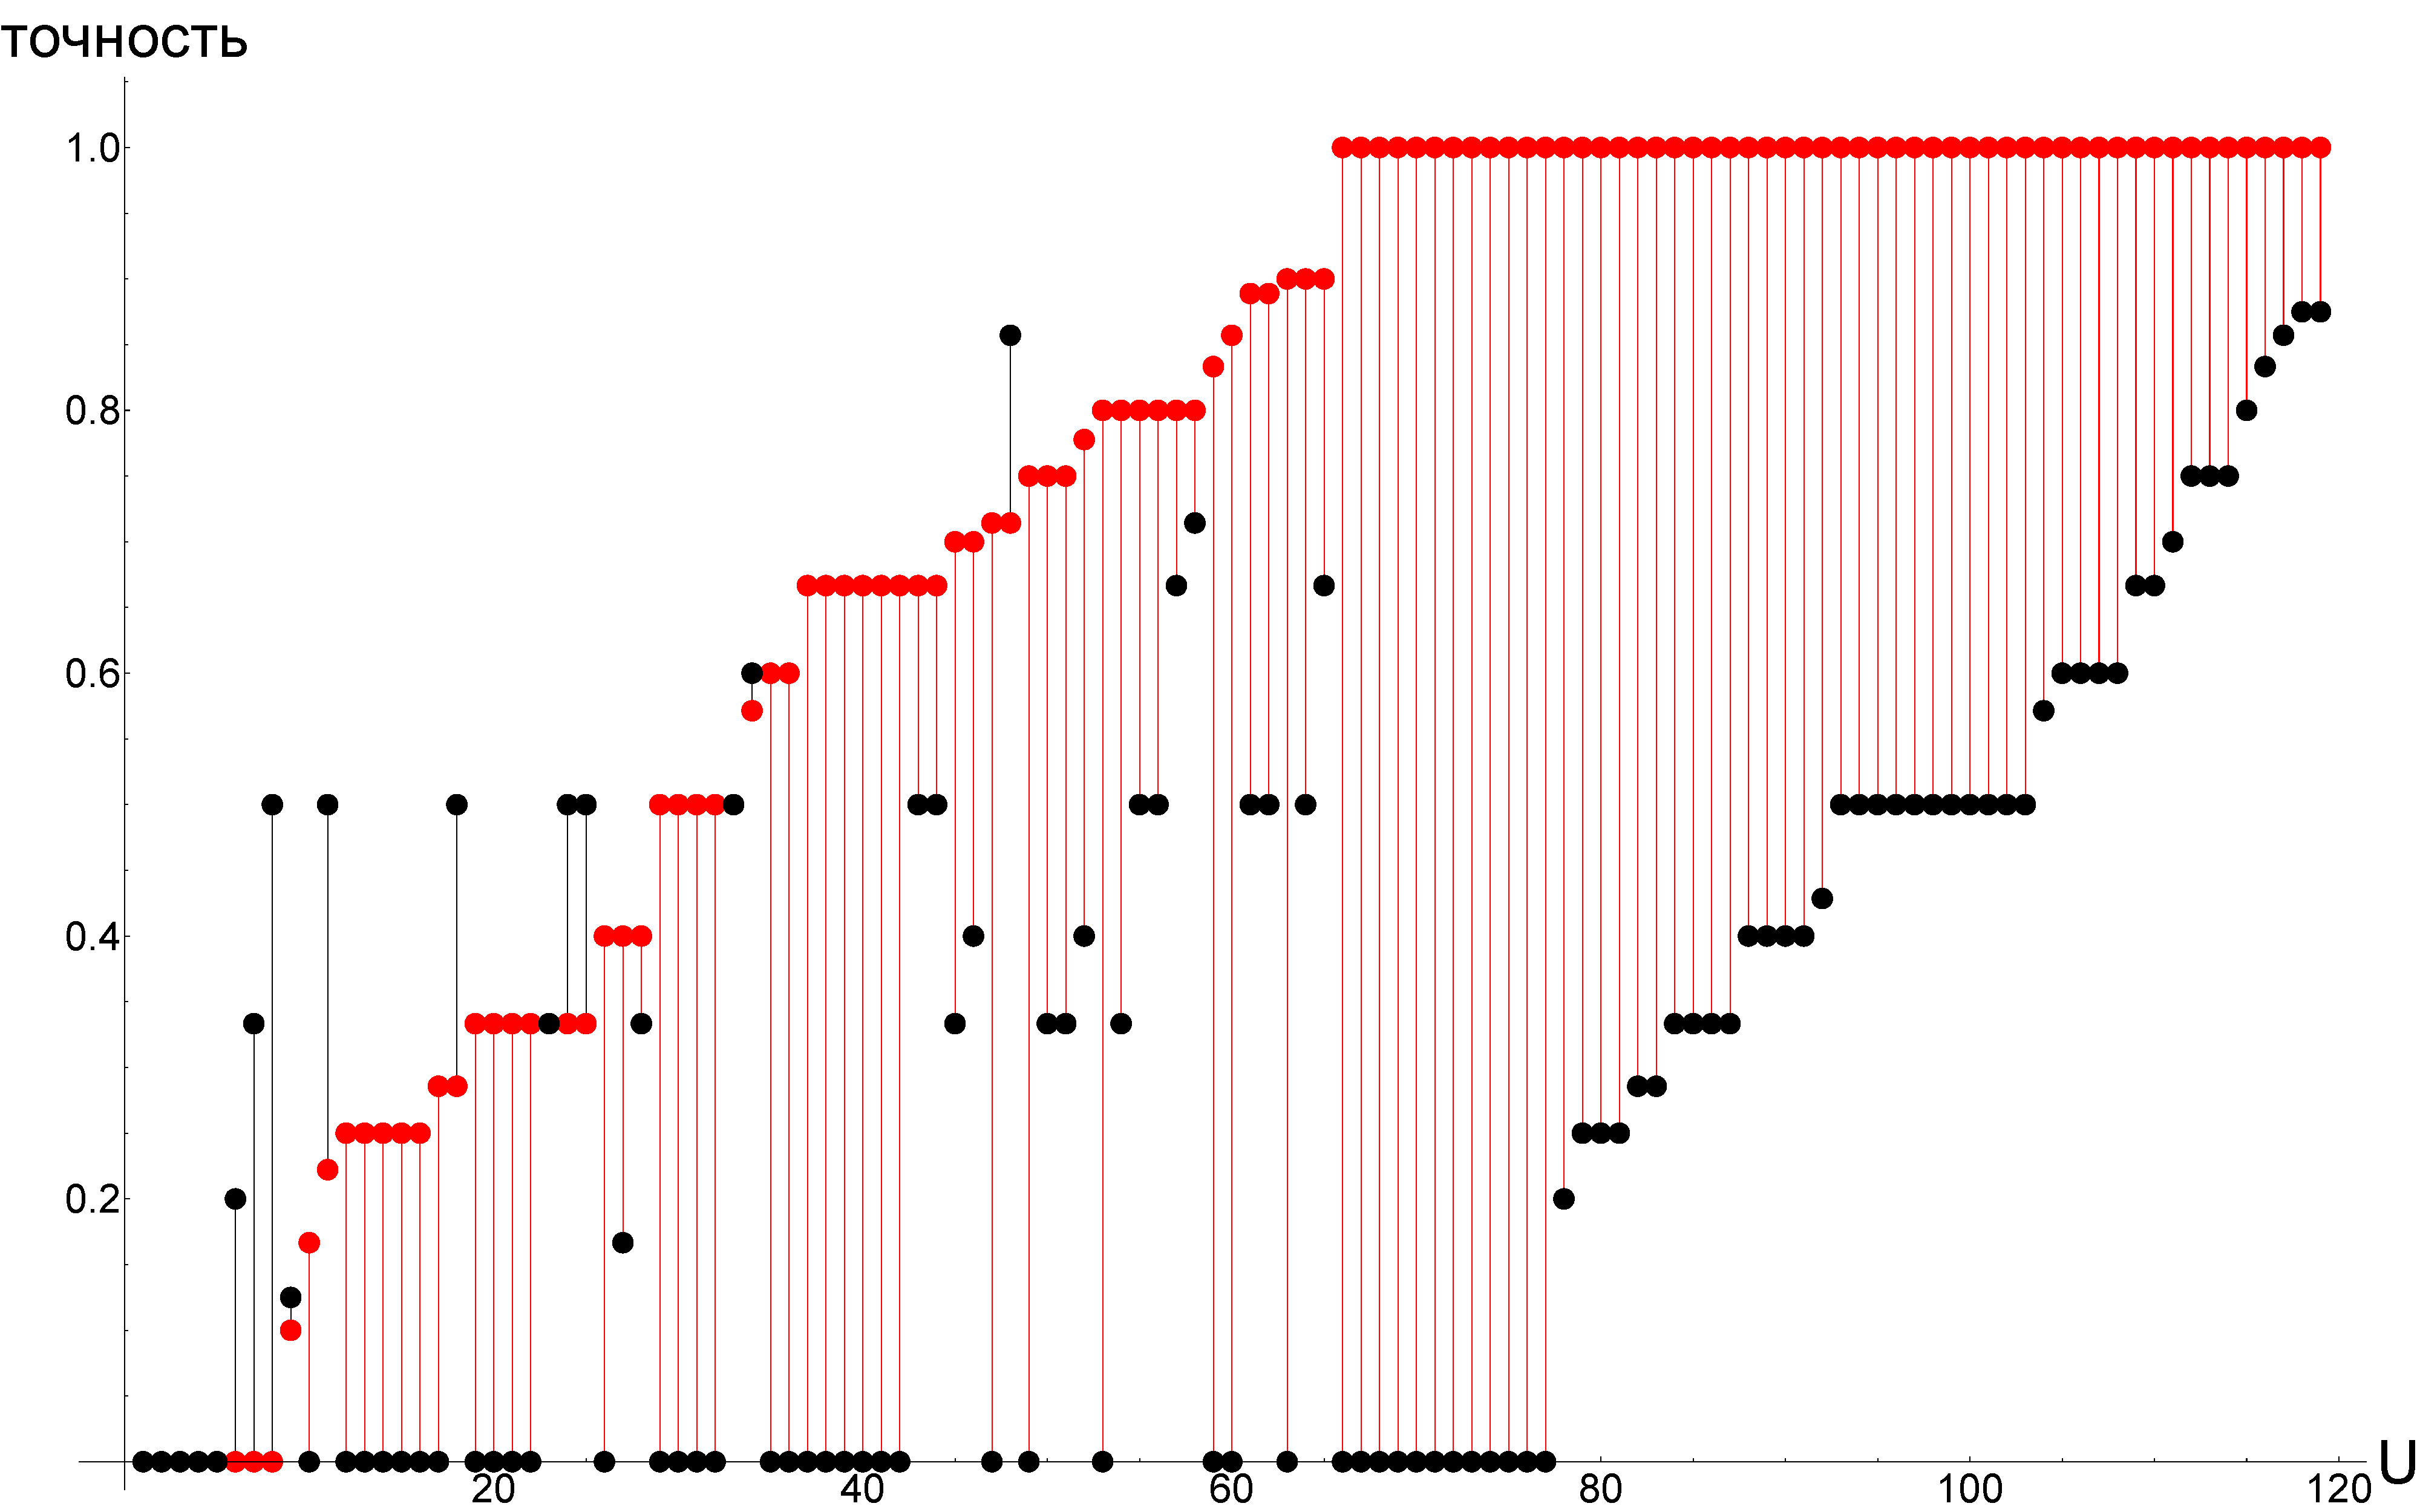
\includegraphics[width=7in,height=4in]{pics/results/ib_method_in_ib_and_fuzzy_model.pdf}
\end{center}
\end{figure}

\begin{table}[H]
	\caption{Средняя точность решений при применении правила вывода $\Pi_{O}$ в нечеткой модели и ООМ}
  \label{tbl:topn_hamming}
  \begin{center}
	\begin{tabular}{|c|c|}
	  \hline
		Модель& Точность \\ \hline
		ООМ&0,627 \\ \hline
		Нечеткая&0,312 \\ \hline
	\end{tabular}
  \end{center}
\end{table}

Практические результаты подтверждают вывод (\ref{trm:fuz-eff-oom}) о том, что
применение $\Pi_O$ в нечеткой модели более эффективно по критерию качества,
чем применение того же правила в АКМ.

\subsubsection{Применение правила вывода нечеткой модели для решения задачи
$topN$}
В данном пункте приведем и сравним результаты решения задачи $topN$, полученные:
\begin{enumerate}
	\item в ООМ:
		\begin{itemize}
			\item
			стандартный алгоритма решения задачи
			$topN$ (\ref{alg:topn-solve-ors}), основанный на
			правиле вывода $\Pi_O$;
			\item
			пороговое значение $\Delta_i$ равно $0,9$;
			\item
		применяемая мера сходства --- косинус угла (\ref{sim-cos})
		между контентами, которые представляются в ООМ в виде векторов.
		\end{itemize}
	\item
		\begin{itemize}
			\item
			алгоритма решения задачи
			$topN$ (\ref{alg:fuz-topn}), основанный на
			правиле вывода $\Pi_f$;
		\end{itemize}
\end{enumerate}


\begin{figure}[H]
	\caption{Качество решений задачи $topN$ при использовании $\Pi_O$ в ООМ и
	$\Pi_f$ в НРС}
	\label{pic:topn_pio_pif}
	\begin{center}
		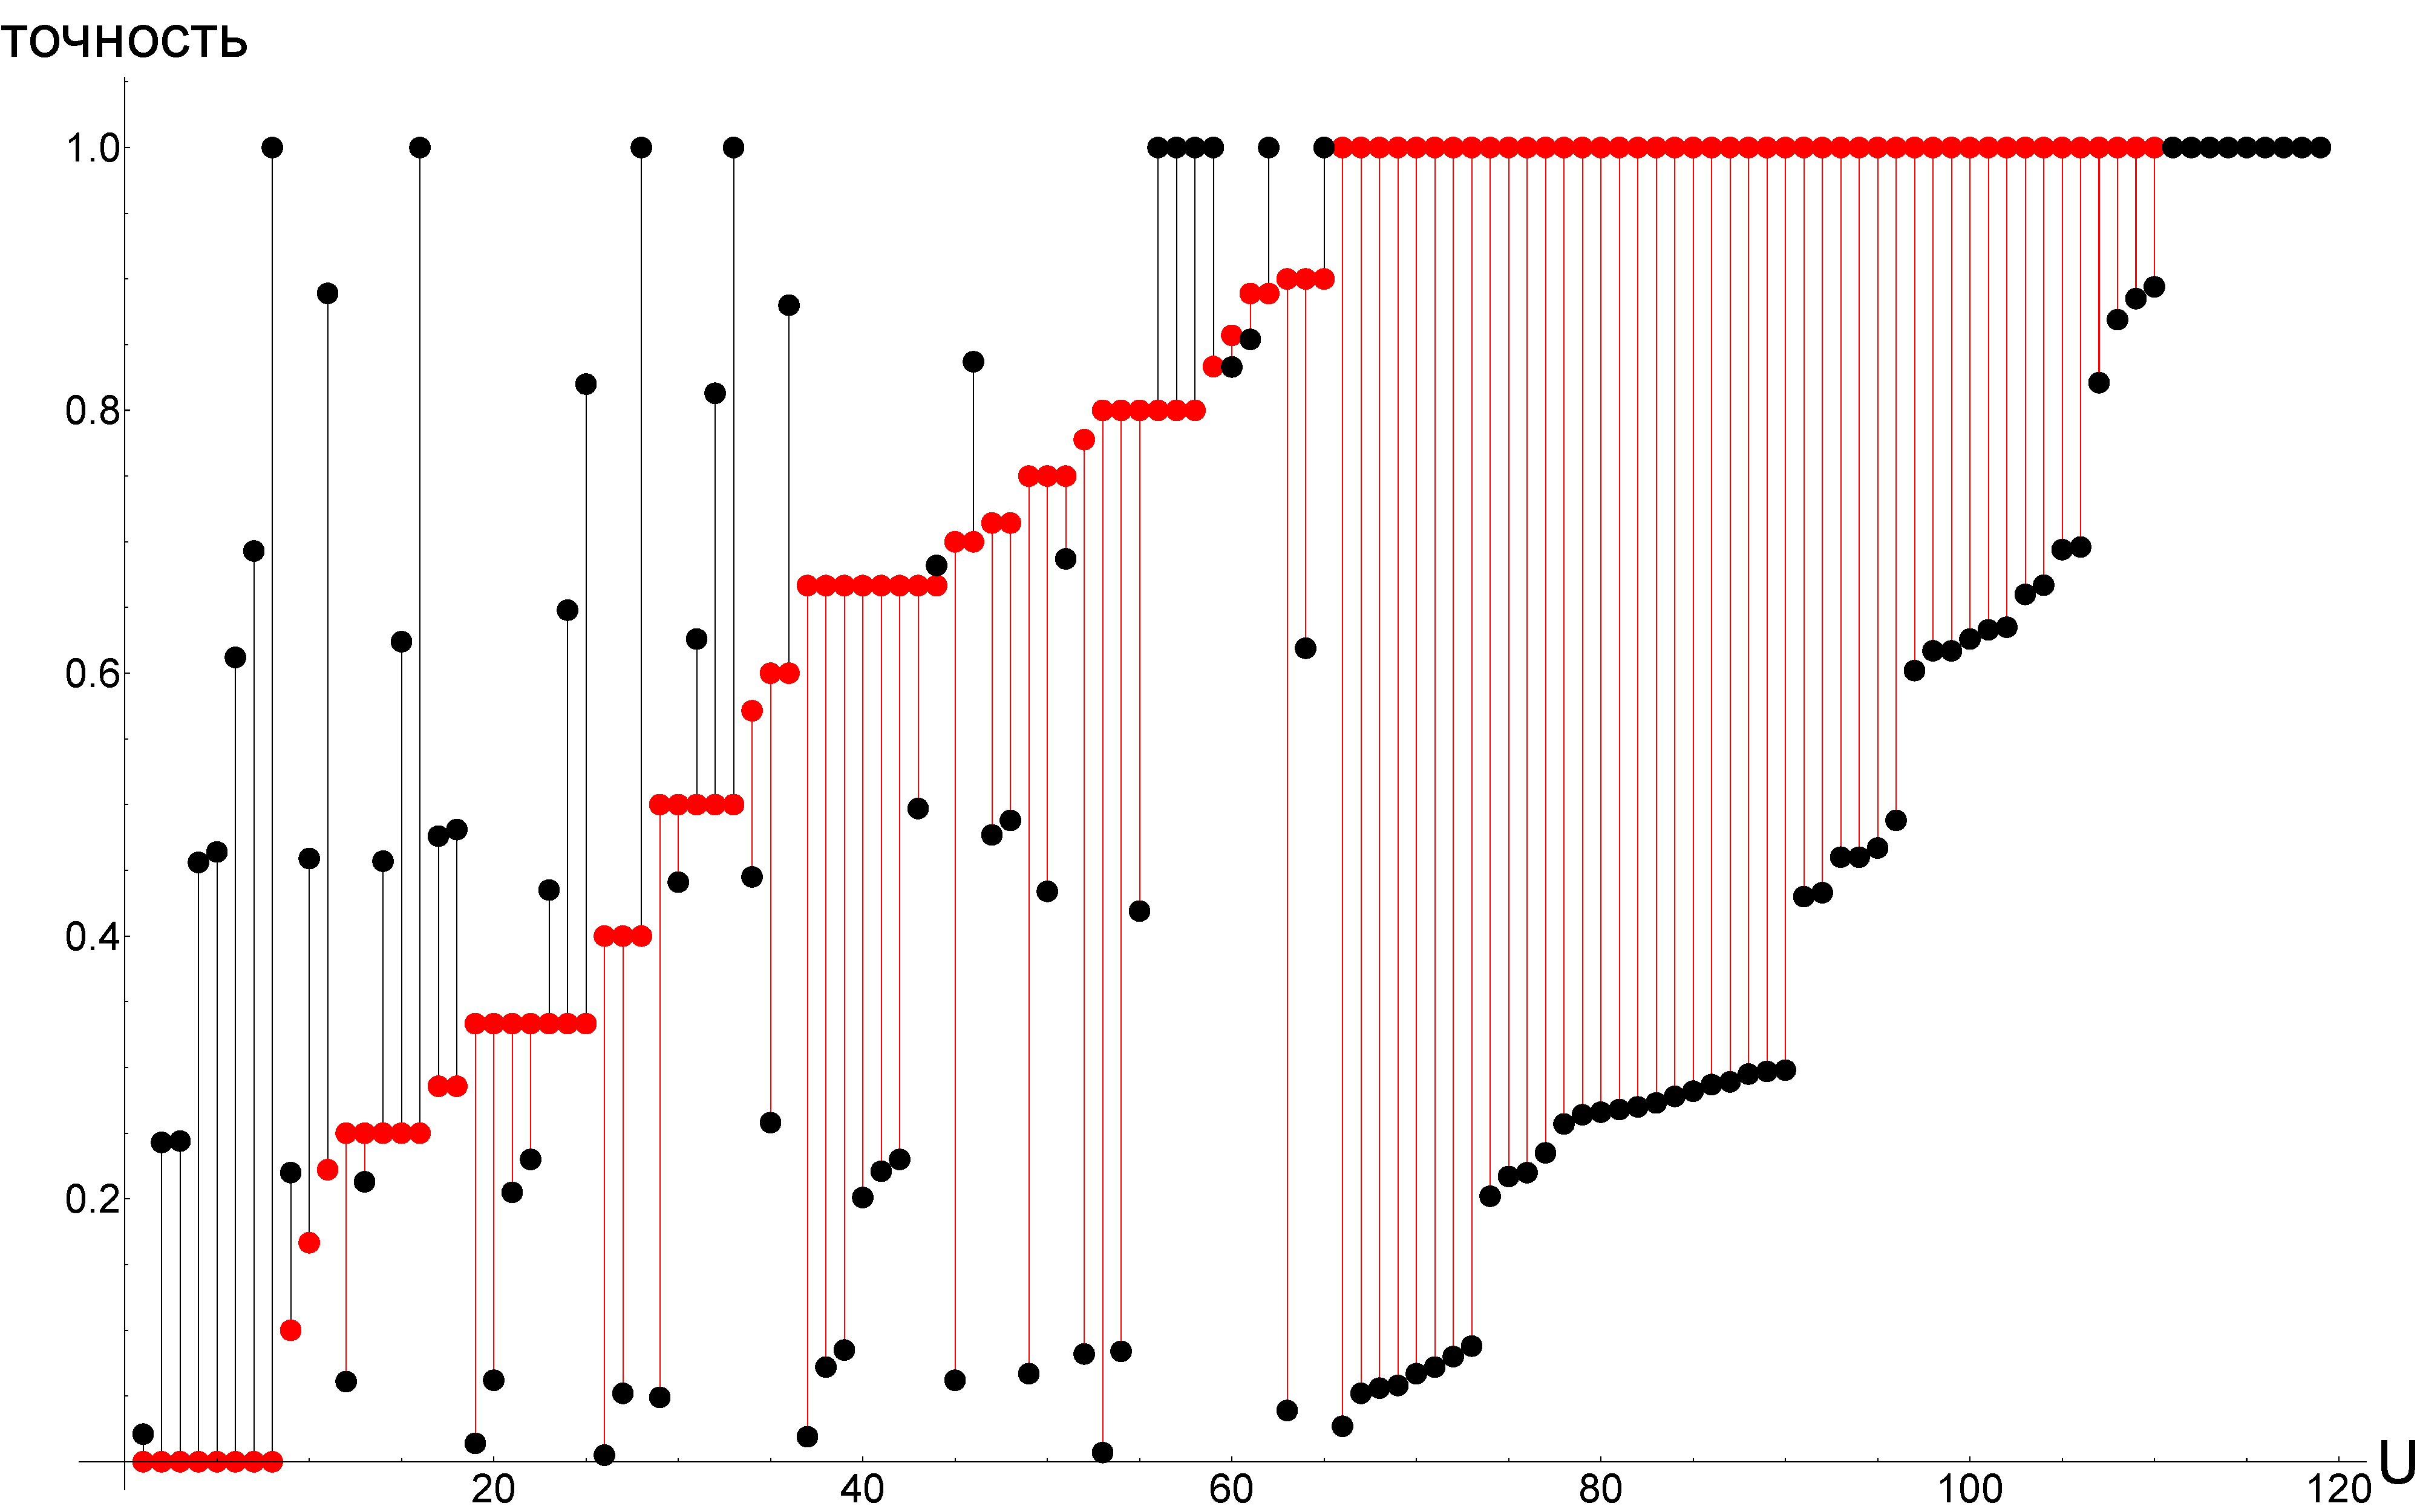
\includegraphics[width=7in,height=4in]{pics/results/topn_oom_fuzz.pdf}
\end{center}
\end{figure}

\begin{table}[H]
	\caption{Средняя точность решений в ООМ и нечеткой модели при применении
	$\Pi_f$}
  \begin{center}
	\label{tbl:topn_fuz}
	\begin{tabular}{|c|c|}
	  \hline
		Модель/Правило вывода & Точность \\ \hline
		ООМ/$\Pi_{O}$&0,627 \\ \hline
		Нечеткая/$\Pi_{f}$&0,420 \\ \hline
	\end{tabular}
  \end{center}
\end{table}


На Рис. \ref{pic:topn_pio_pif} приведены результаты решения
задачи $topN$ при применении $\Pi_O$ в ООМ и нечеткой модели.
Черным цветом обозначены результаты решения в нечеткой модели.
Видно, что в большинстве случаев нечеткая модель более эффективна
по критерию качества. В обратных ситуациях предпочтения пользователя
неоднородны, и $\delta_c$ для таких пользователей определена так, что
$|\rho(u, i) - \rh(u, i)| > \varepsilon_p$.

Практические результаты подтверждают вывод (\ref{trm:fuz-eff-extension}) о том,
что нечеткая модель является эффективным расширением АКМ по критерию качества.


\subsection{Задача прогнозирования}
Результаты представляются графиком и таблицей для каждого пункта.
Координатой оси $X$ является идентификатор пользователя, координатой
оси $Y$ является значение оценки качества.
В качестве функции $\eit$ использовалась функция
NMAE \ref{nmae}.
Другие функции рассматривались так же, но между
функциями одного класса существует корреляция и приведение других графиков
оказывается избыточным.

На графиках представляются данные по двум методам тестирования. Для наглядности
результирующие данные были отсортированы по значениям оценки качества,
принадлежащим первому методу (в каждой паре точек, которые находятся на одной
вертикали, идентификаторы пользователей совпадают).

В таблицах представлены средние значения оценок точности по всем пользователям.

Для проведения тестов данного пункта исходные данные были
стандартно разбиты на тестовое и обучающее множество по следующему принципу:
разбиение проводилось случайно, в обучающее множество входит
80\% данных, в тестовое --- оставшиеся 20\%. В тестировании участвовало
подмножество $P^{\prime} \subset P, P^{\prime} = \{(u, i, \rho(u, i)):
\rho(u, i) = 1\}$.

\subsubsection{Влияние свойства транзитивности на СОМ при решении задачи
прогнозирования}
В данном пункте приведем и сравним результаты решения задачи $pred$, полученные:
\begin{enumerate}
	\item  в СОМ при следующих параметрах:
		\begin{itemize}
			\item
			стандартный алгоритма решения задачи
			$pred$ (\ref{alg:p-srs}), основанный на
			правиле вывода $\Pi_C$;
			\item
			пороговое значение $\Delta_u$ равно $0,9$;
			\item
		применяемая мера сходства --- коэффициент корреляции Пирсона
				(\ref{pearson}).
		\end{itemize}
	\item  в СОМ при следующих параметрах:
		\begin{itemize}
			\item
			стандартный алгоритма решения задачи
			$pred$ (\ref{alg:p-srs}), основанный на
			правиле вывода $\Pi_C$;
			\item
			пороговое значение $\Delta_u$ равно $0,49$;
			\item
		применяемая мера сходства --- коэффициент корреляции Пирсона
				(\ref{pearson}).
		\end{itemize}
\end{enumerate}

При $\Delta_u = 0,9$ вероятность того, что $(u \rt v) \wedge (v \rt z)
\Rightarrow (u \rt z)$, выше, чем при $\Delta_u = 0,49$.
На Рис. \ref{pic:predtrans} приведены результаты решений задачи $topN$ при
различных пороговых значениях. Черным цветом приведены результаты для
$\Delta_u = 0,9$, красным --- для $\Delta_u = 0,49$.
Видно, что при $\Delta_u = 0,9$ результаты решений эффективней, так
как большинство точек, соответствующих $\Delta_u = 0,9$ проходит ниже точек,
соответствующих $\Delta_u = 0,49$, что также подтверждается табличными данными,
представленными в таблице (\ref{tbl:predtrans}).

Некоторые результаты при $\Delta_u = 0,9$ хуже, чем при
$\Delta_u = 0,49$. Это происходит для тех пользователей,
для которых характерно свойство неоднородности.

\begin{figure}[H]
	\caption{Влияние свойства транзитивности на СОМ при решении задачи $pred$}
	\label{pic:predtrans}
	\begin{center}
		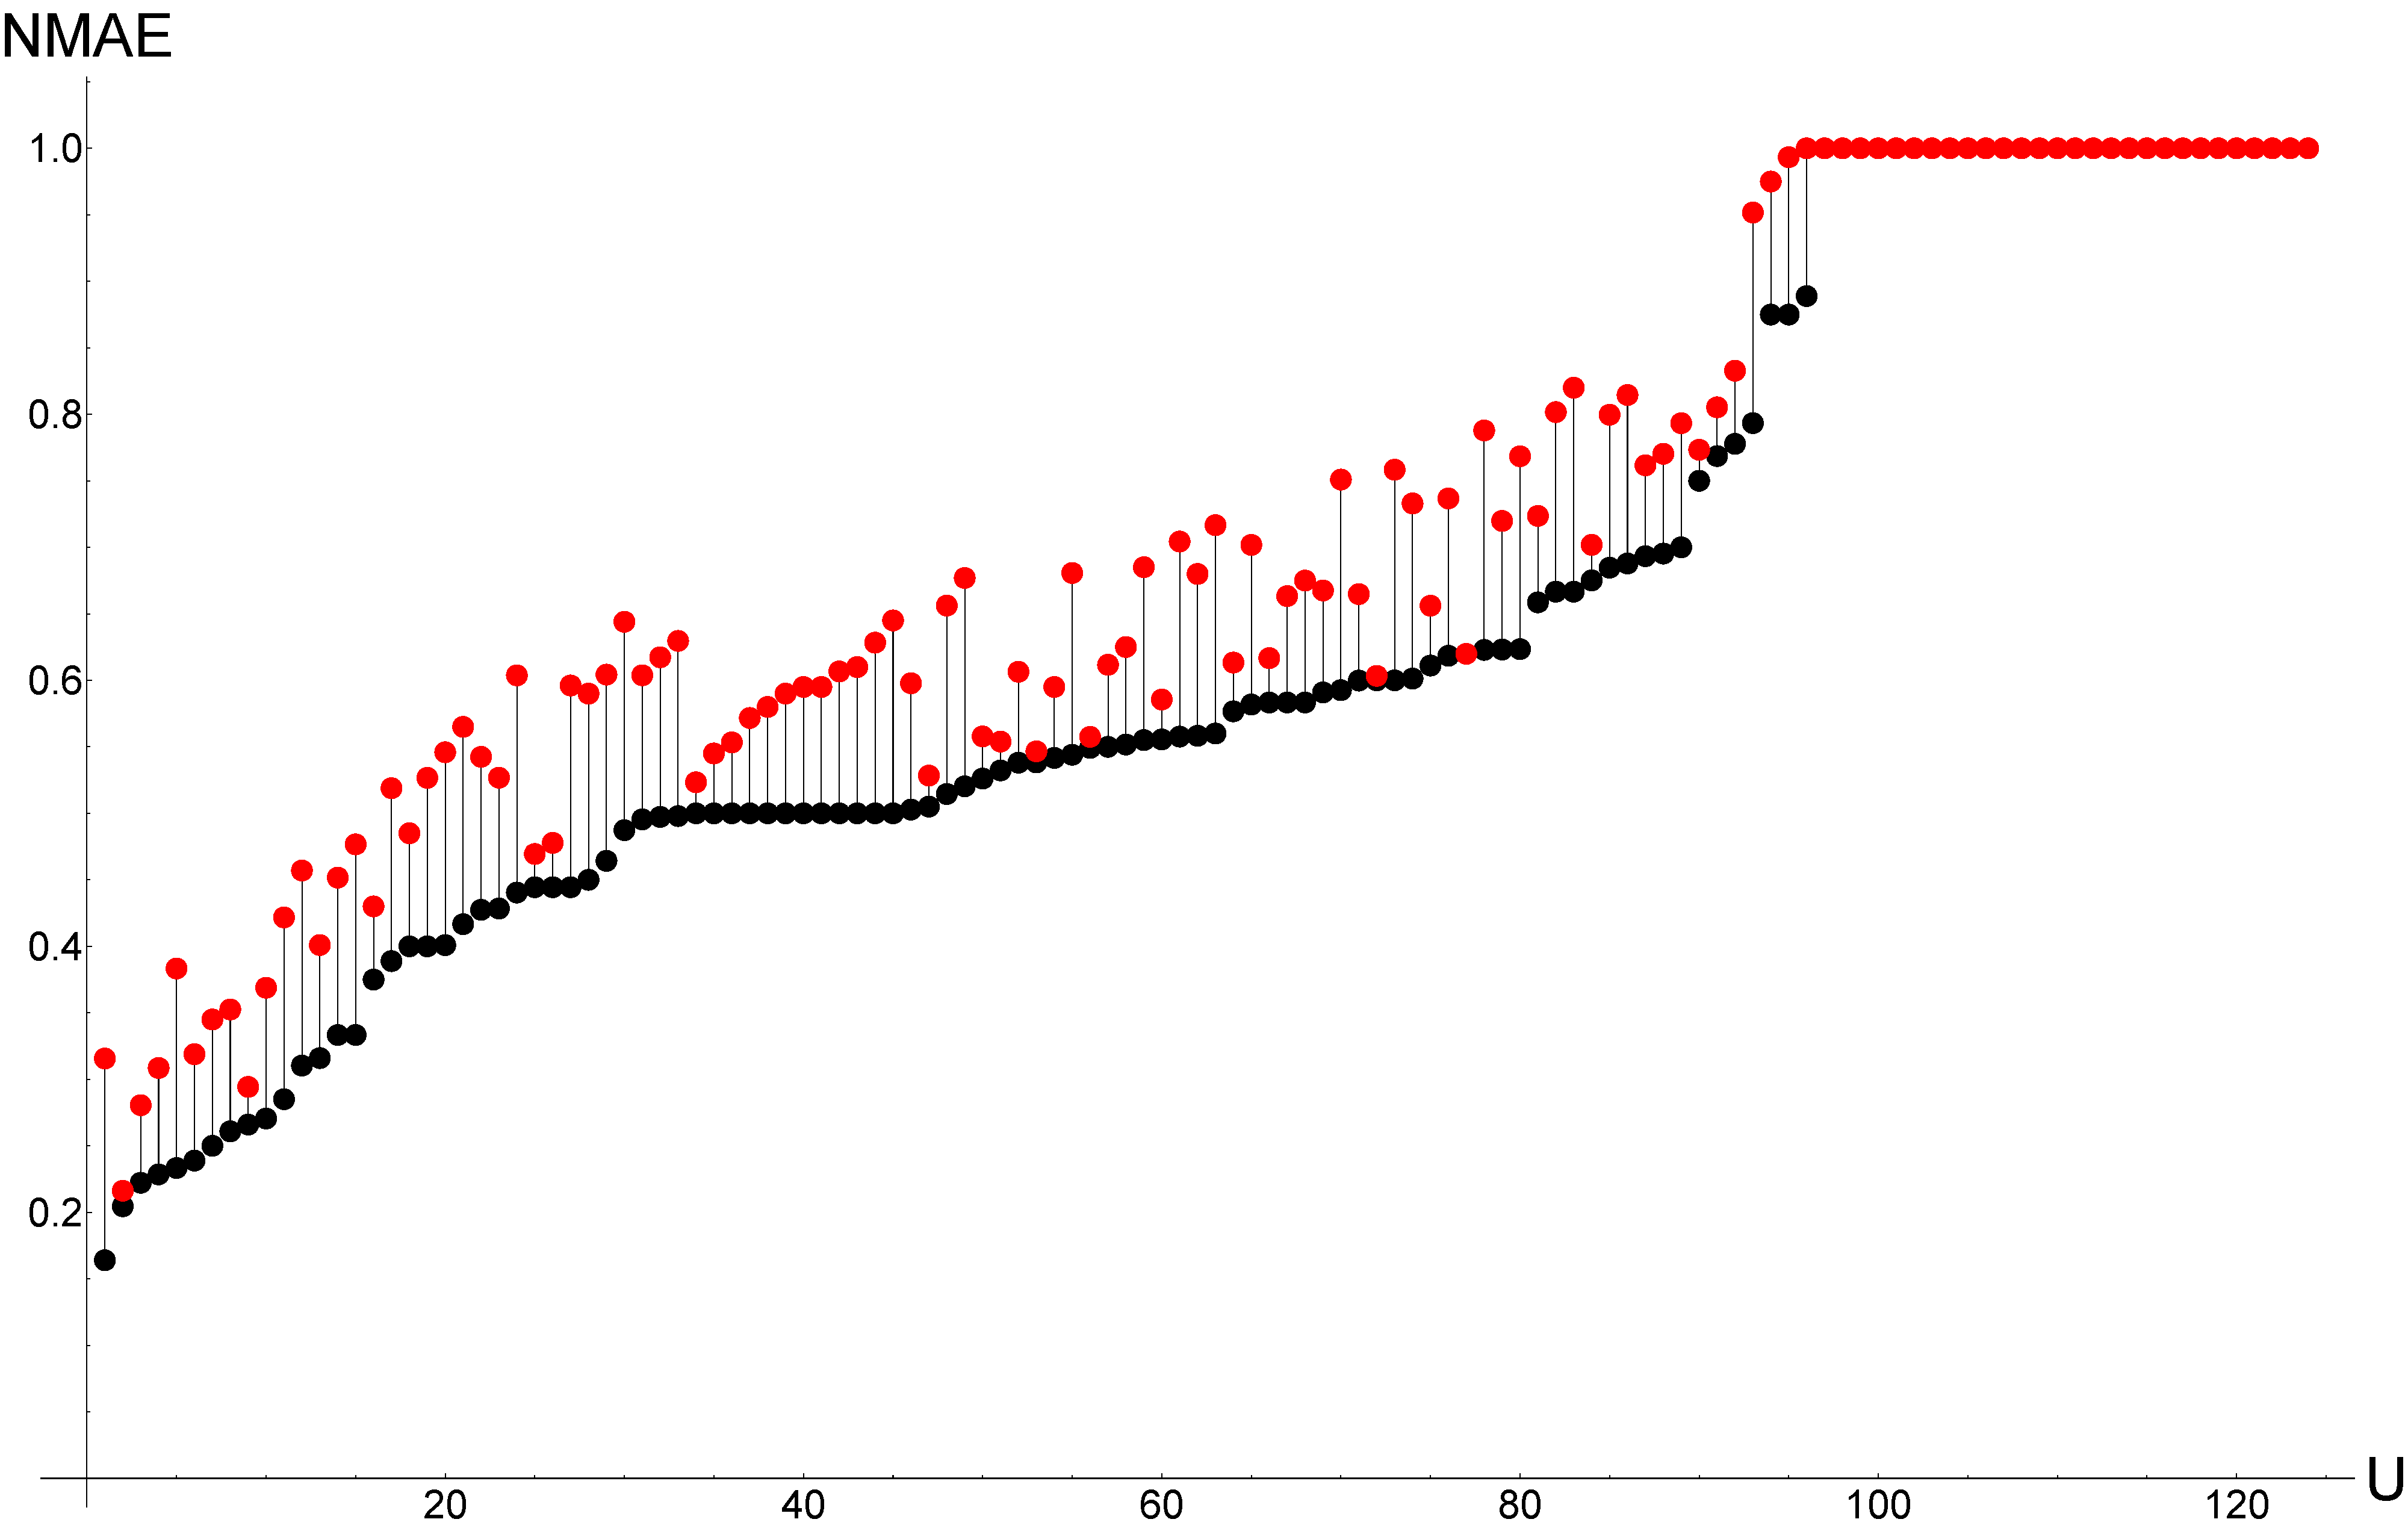
\includegraphics[width=7in,height=4in]{pics/results/ub_transitivity.pdf}
\end{center}
\end{figure}

\begin{table}[H]
	\caption{Влияние свойства транзитивности на СОМ при решении задачи $pred$}
  \label{tbl:predtrans}
  \begin{center}
	\begin{tabular}{|c|c|}
	  \hline
		Пороговое значение & NMAE \\ \hline
		0,9&0,495 \\ \hline
		0,49&0,601 \\ \hline
	\end{tabular}
  \end{center}
\end{table}

\subsubsection{Применение правила вывода СОМ в коллаборативной и нечеткой
моделях}
В данном пункте приведем и сравним результаты решения задачи $topN$, полученные:
\begin{enumerate}
	\item  в СОМ при следующих параметрах:
		\begin{itemize}
			\item
			стандартный алгоритма решения задачи
			$pred$ (\ref{alg:p-srs}), основанный на
			правиле вывода $\Pi_C$;
			\item
			пороговое значение $\Delta_u$ равно $0,9$;
			\item
		применяемая мера сходства --- коэффициент корреляции Пирсона
		\end{itemize}
	\item в нечеткой при следующих параметрах:
		\begin{itemize}
			\item
			стандартный алгоритма решения задачи
			$pred$ (\ref{alg:p-srs}), основанный на
			правиле вывода $\Pi_C$;
			\item
				применяемая мера сходства --- обобщенное расстояние Хэмминга
				(\ref{fuz:rhi})
		\end{itemize}
\end{enumerate}

На Рис. \ref{pic:predpio} приведены результаты решения
задачи $topN$ при применении $\Pi_C$ в СОМ и нечеткой модели.
Черным цветом обозначены результаты решения в нечеткой модели.
Видно, что в большинстве случаев нечеткая модель более эффективна
по критерию качества. В обратных ситуациях предпочтения пользователя
неоднородны.
%, и $\delta_c$ для таких пользователей определена так, что
%$|\rho(u, i) - \rh(u, i)| > \varepsilon_p$.

\begin{figure}[H]
	\caption{Качество решений при применении правила вывода $\Pi_{C}$ в нечеткой модели и СОМ}
	\label{pic:predpio}
	\begin{center}
		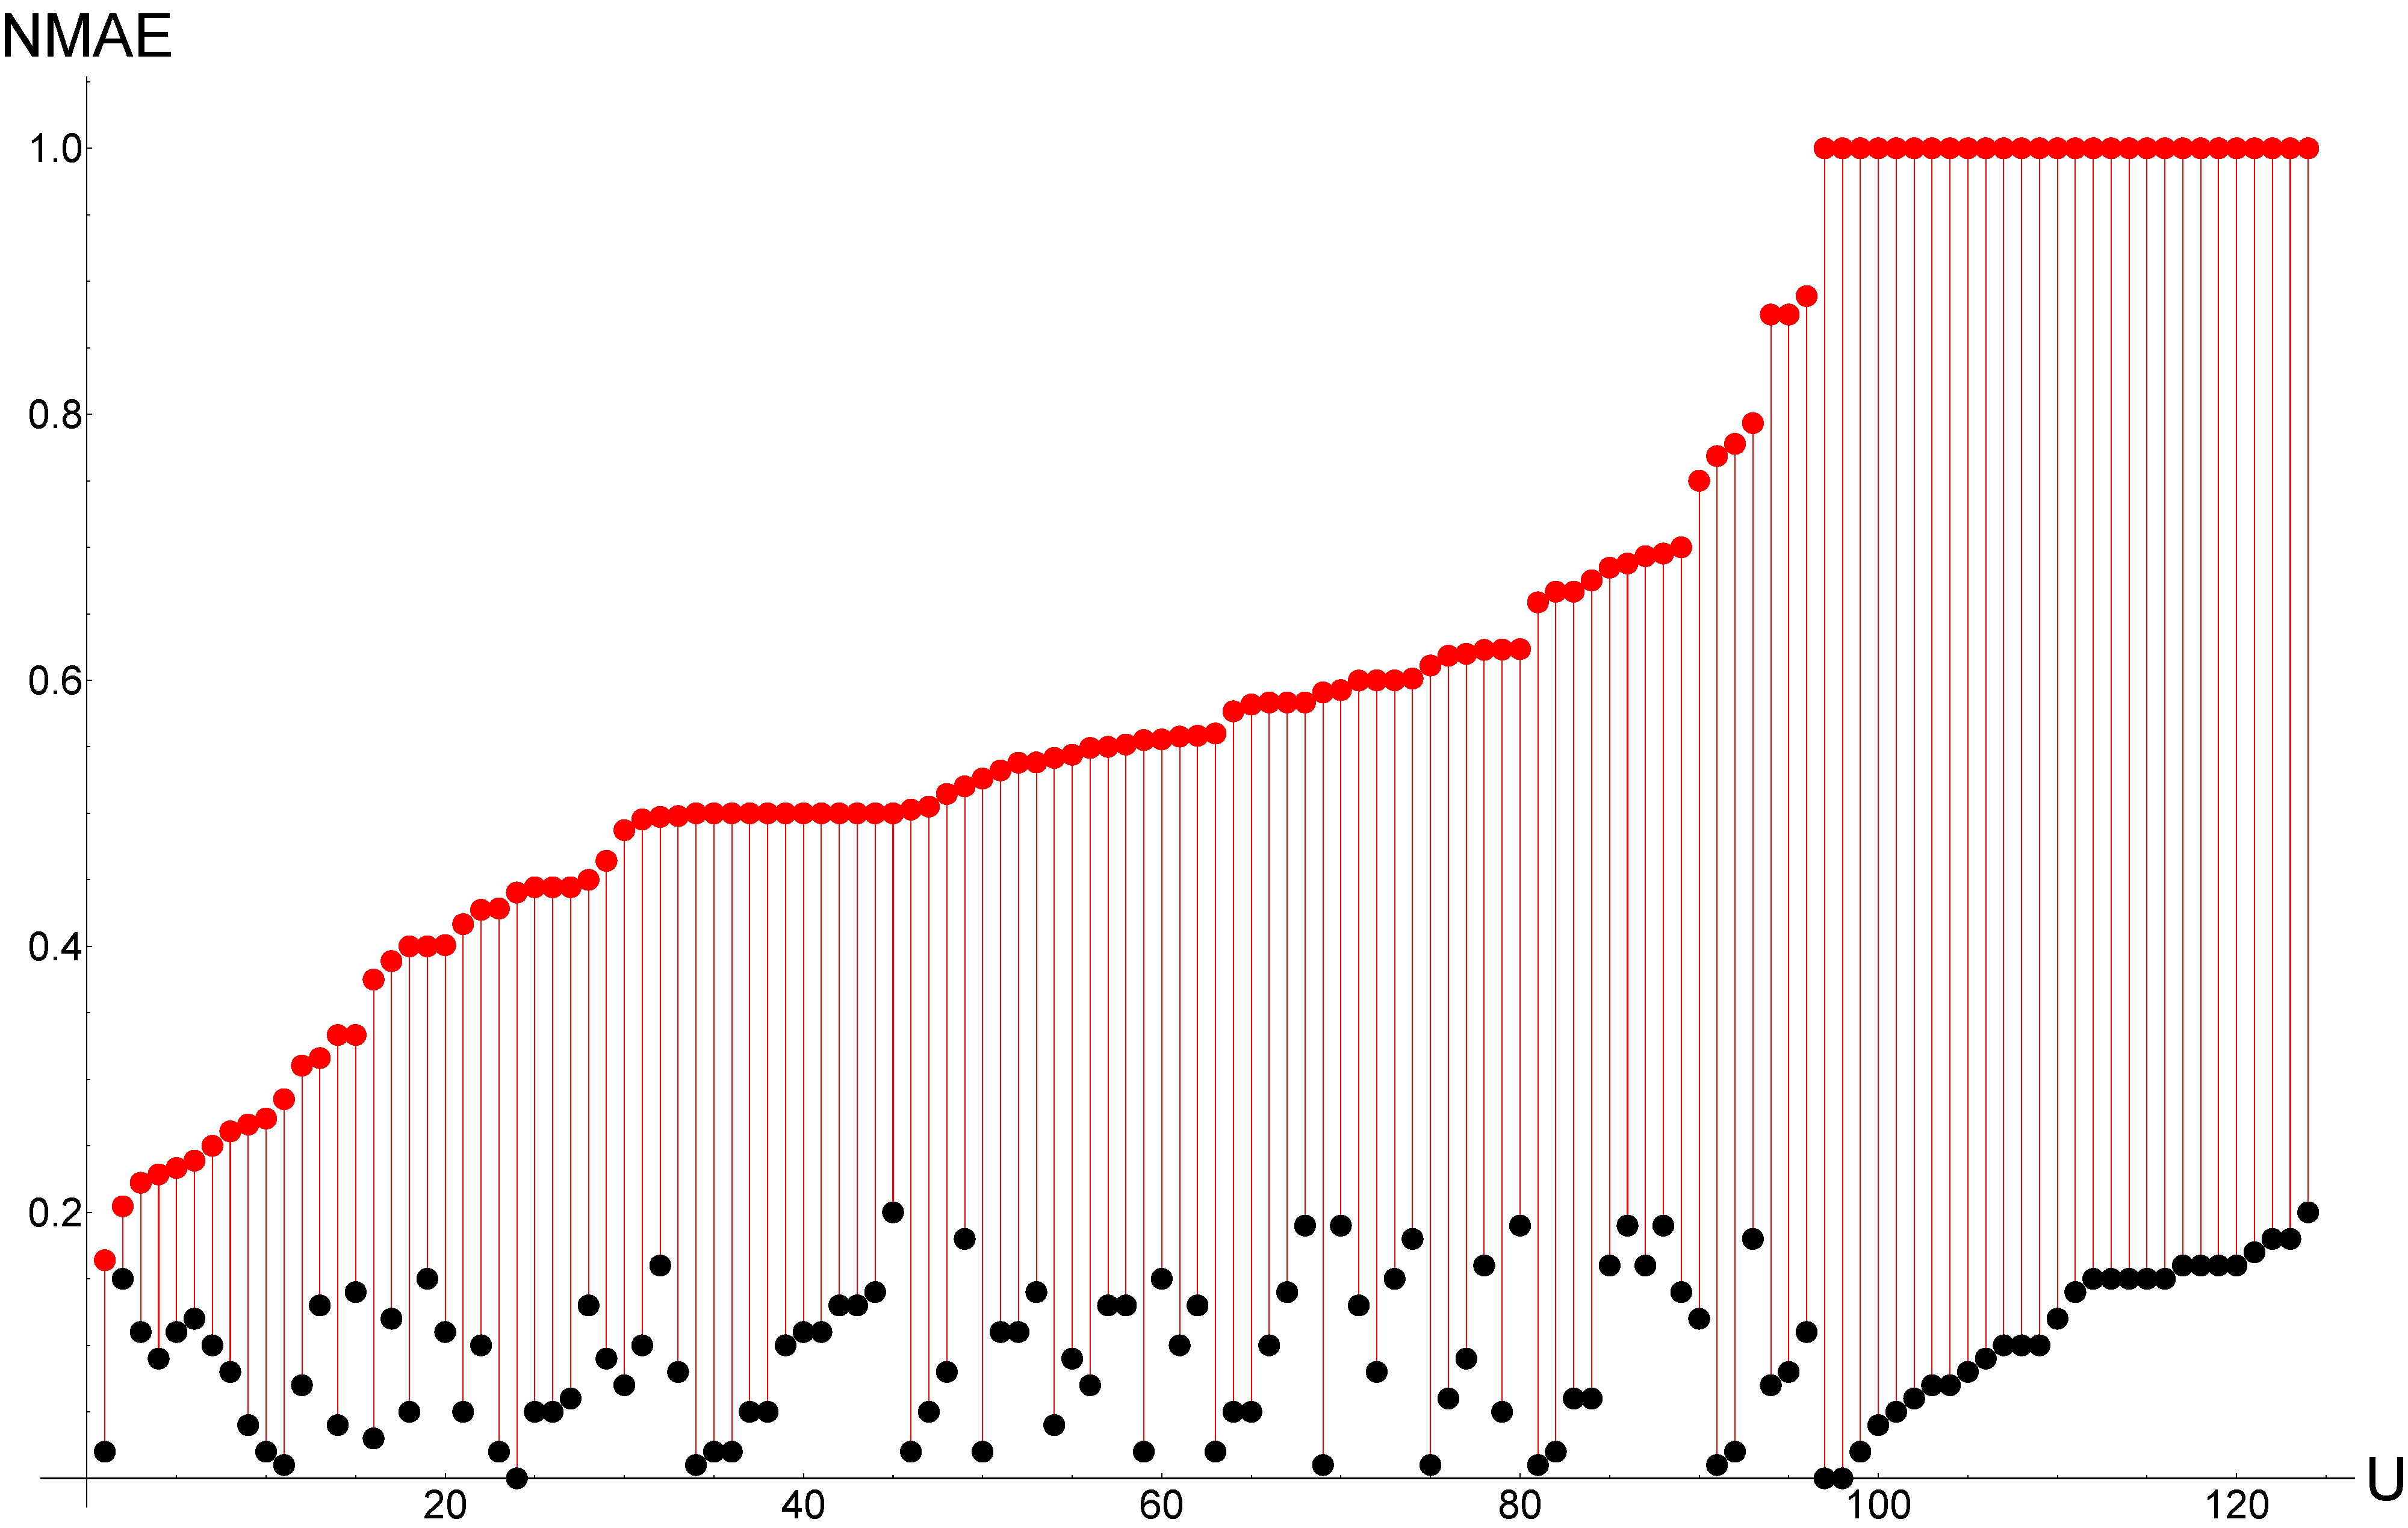
\includegraphics[width=7in,height=4in]{pics/results/ub_method_in_ub_and_fuzz_model.pdf}
\end{center}
\end{figure}

\begin{table}[H]
	\caption{Средняя точность решений при применении правила вывода $\Pi_{C}$ в нечеткой модели и СОМ}
  \label{tbl:predhamming}
  \begin{center}
	\begin{tabular}{|c|c|}
	  \hline
		Модель& Точность \\ \hline
		Нечеткая&0,001 \\ \hline
		COM&0,495\\ \hline
	\end{tabular}
  \end{center}
\end{table}

Практические результаты подтверждают вывод (\ref{trm:fuz-eff-com}) о том, что
применение $\Pi_C$ в нечеткой модели более эффективно по критерию качества,
чем применение того же правила в АКМ.

\subsubsection{Применение правила вывода нечеткой модели для решения задачи
$pred$}
В данном пункте приведем и сравним результаты решения задачи $pred$, полученные:
\begin{enumerate}
	\item в СОМ:
		\begin{itemize}
			\item
			стандартный алгоритма решения задачи
			$topN$ (\ref{alg:topn-solve-ors}), основанный на
			правиле вывода $\Pi_C$;
			\item
			пороговое значение $\Delta_u$ равно $0,9$;
			\item
		применяемая мера сходства --- косинус угла (\ref{sim-cos})
		между контентами, которые представляются в СОМ в виде векторов.
		\end{itemize}
	\item
		\begin{itemize}
			\item
			алгоритма решения задачи
			$pred$ (\ref{alg:fuz-p}), основанный на
			правиле вывода $\Pi_f$;
		\end{itemize}
\end{enumerate}


\begin{figure}[H]
	\caption{Качество решений задачи $pred$ при использовании $\Pi_C$ в СОМ и
	$\Pi_f$ в нечеткой модели}
	\label{pic:predpio_pif}
	\begin{center}
		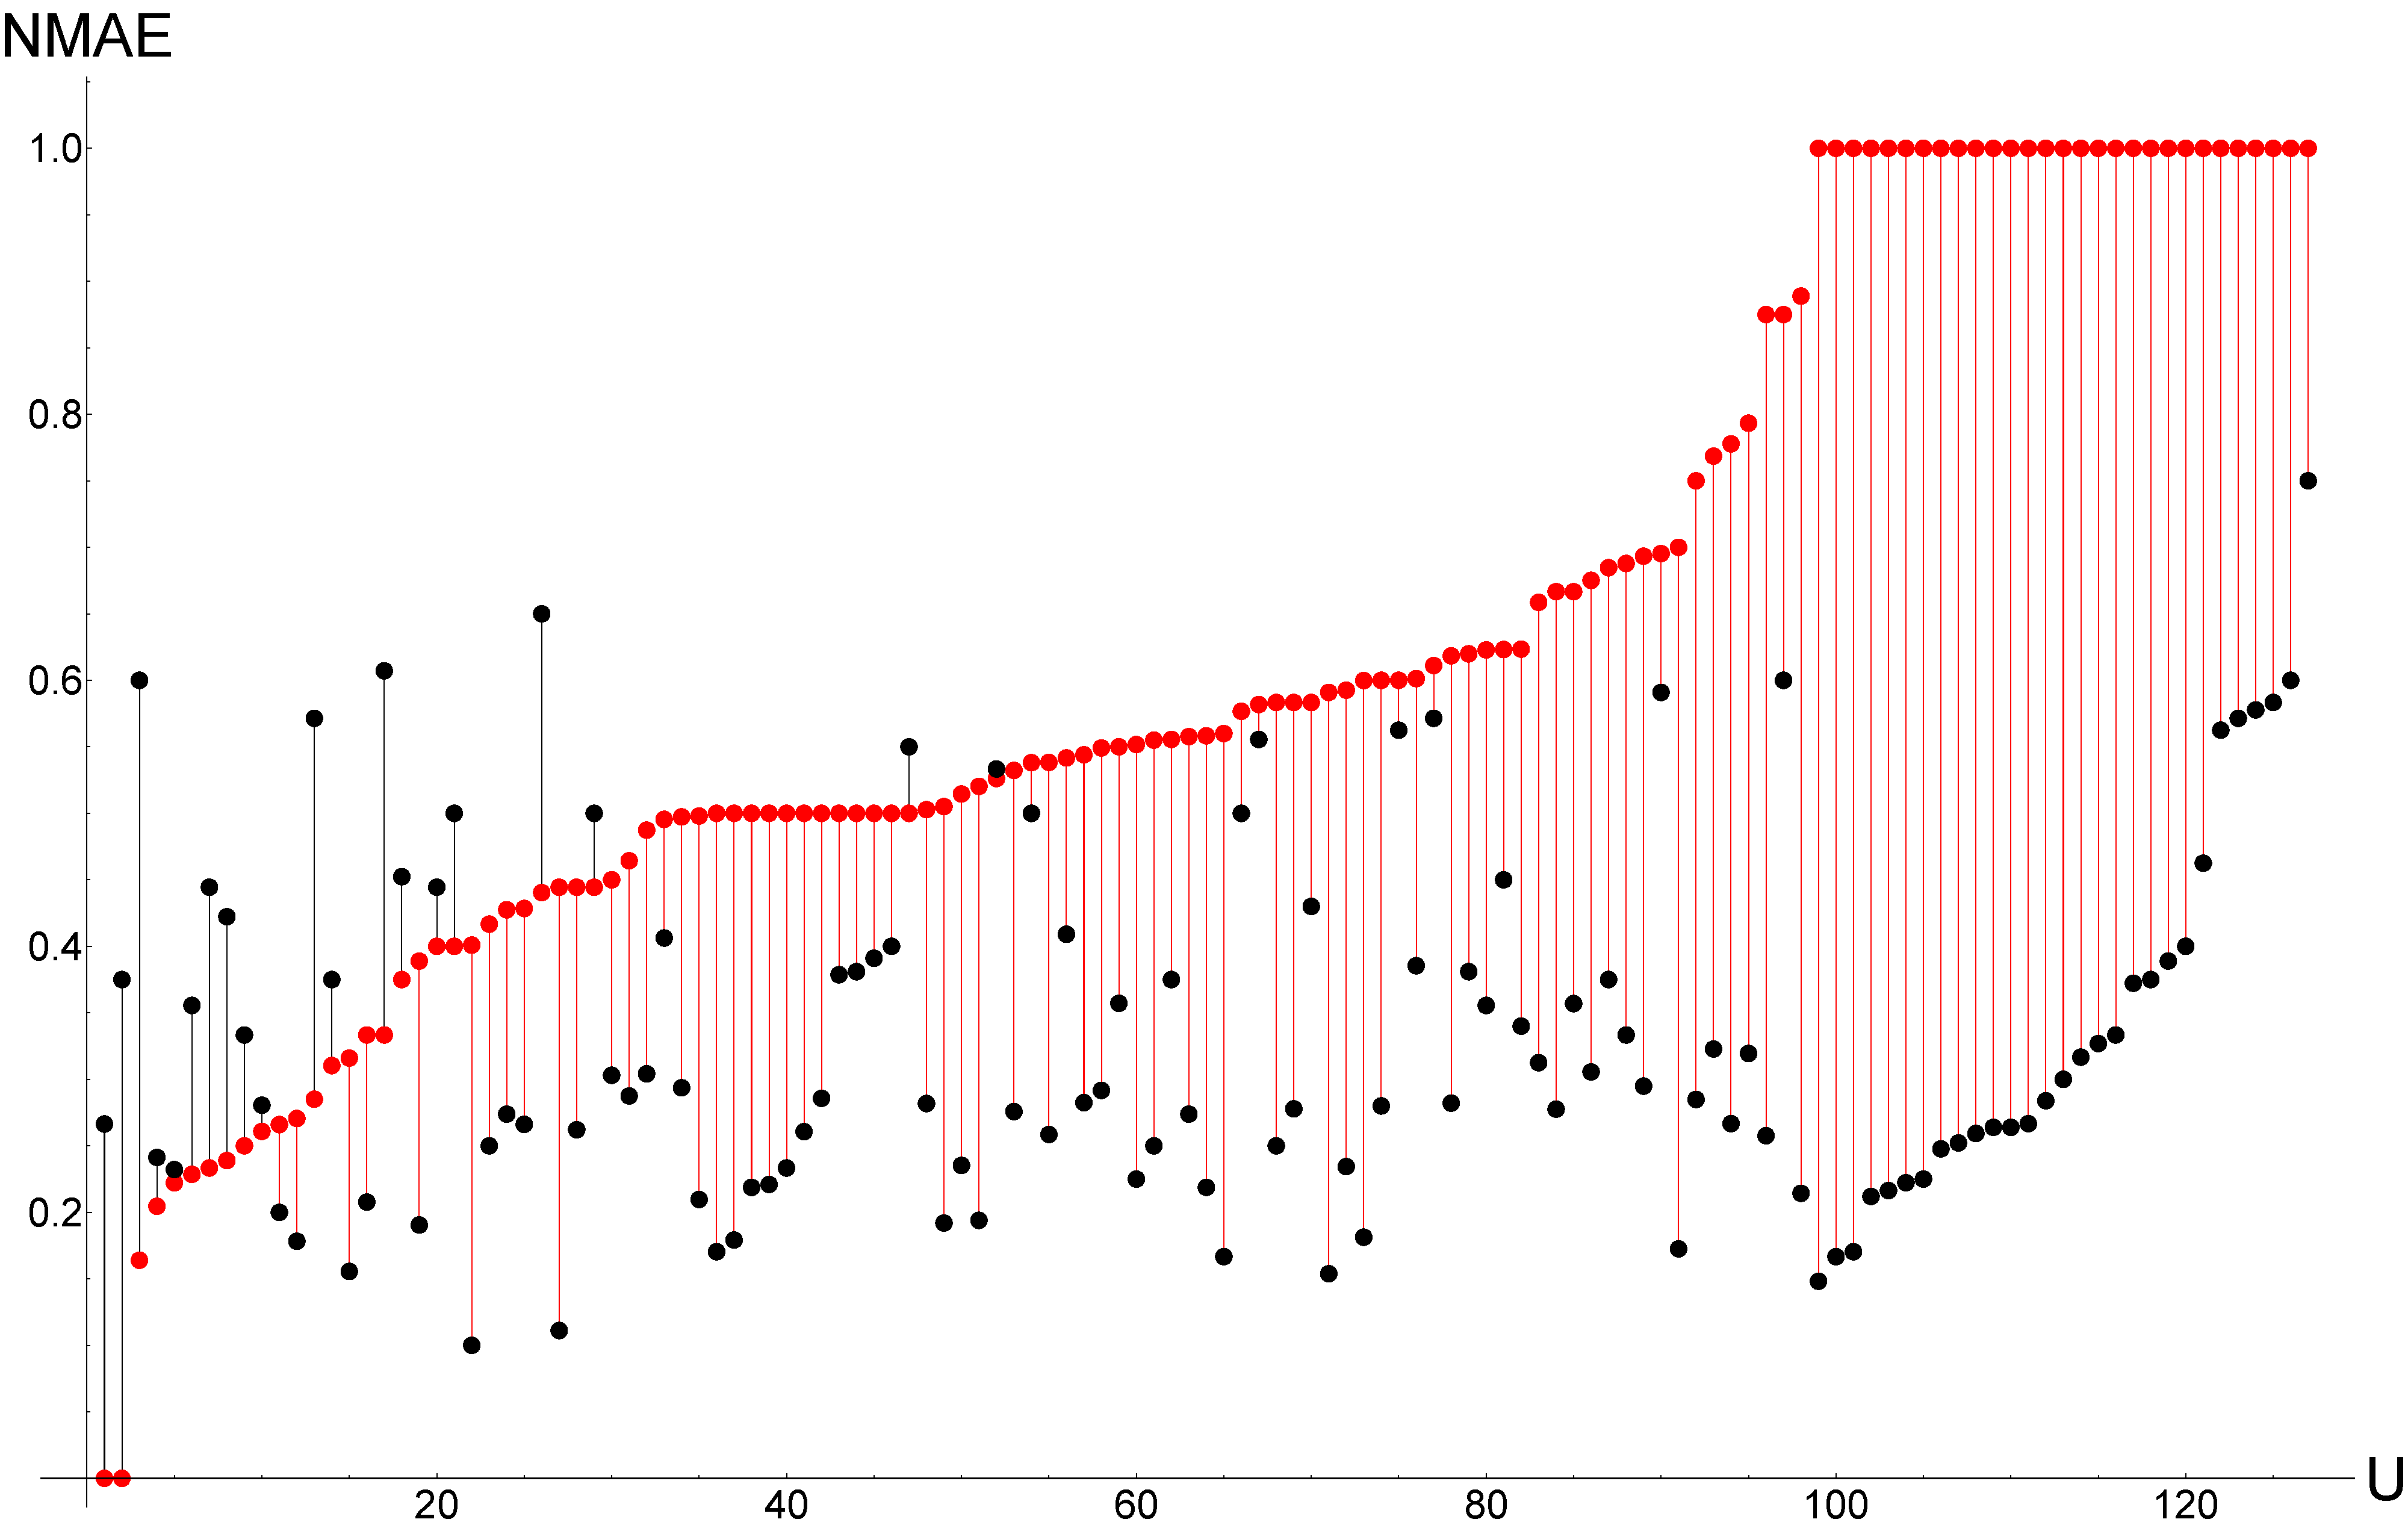
\includegraphics[width=7in,height=4in]{pics/results/ub_vs_fuzzy.pdf}
\end{center}
\end{figure}

\begin{table}[H]
	\caption{Средняя точность решений в СОМ и нечеткой модели при применении
	$\Pi_f$}
  \begin{center}
	\label{tbl:predfuz}
	\begin{tabular}{|c|c|}
	  \hline
		Модель/Правило вывода & Точность \\ \hline
		СОМ/$\Pi_{O}$&0,495\\ \hline
		Нечеткая/$\Pi_{f}$&0,334 \\ \hline
	\end{tabular}
  \end{center}
\end{table}


На Рис. \ref{pic:predpio_pif} приведены результаты решения
задачи $pred$ при применении $\Pi_C$ в СОМ и нечеткой модели.
Черным цветом обозначены результаты решения в нечеткой модели.
Видно, что в большинстве случаев нечеткая модель более эффективна
по критерию качества. В обратных ситуациях предпочтения пользователя
неоднородны, и $\delta_c$ для таких пользователей определена так, что
$|\rho(u, i) - \rh(u, i)| > \varepsilon_p$.

Практические результаты подтверждают вывод (\ref{trm:fuz-eff-extension}) о том,
что нечеткая модель является эффективным расширением АКМ по критерию качества.


%
\section{Сравнение моделей по критерию стабильности}
\subsection{Влияние свойства динамики исходных данных}

В аналитической главе говорилось о влиянии свойства динамики
данных (\ref{ass:dynamic}) на качество решения в СОМ, а точнее на выполнение
эвристического утверждения СОМ (\ref{srs-assert}). Для теста данного пункта
была произведена имитация проявления свойства динамики, для этого
исходные данные были разбиты не стандартно в пропорции 80 к 20, а
в пропорции 40 к 60, то есть в обучающее множество попало 40\%
данных, остальные --- в тестовое. При таком разбиении вероятность
того, что $u \ru v$ на обучающем множестве выполняется, но на тестовом --- нет,
высока.


Результаты представлены в следующих формах:
\begin{enumerate}
	\item таблицей <<Влияние свойства динамики на качество решения при применении
	$\Pi_C$ в СОМ>> (\ref{tbl:dynamic-com}), в которой указаны
	средние значения $NMAE$ при решении задачи прогнозирования
	в СОМ и при использовании стандартного алгоритма
	на стандартно разбиении и на разбиении 40/60. Значения
	$NMAE$ для разбиения 40/60 выше, что говорит о зависимости
	качества решения от выполнения эвристического утверждения и его
		зависимости от свойств исходных данных;

	\item таблицей <<Влияние свойства динамики на качество решения при применении
	$\Pi_C$ в нечеткой модели>> (\ref{tbl:dynamic-com}), в которой указаны
	средние значения $NMAE$ при решении задачи прогнозирования
	в нечеткой модели и при использовании стандартного алгоритма
	на стандартно разбиении и на разбиении 40/60. Значения
	$NMAE$ для разбиения 40/60 выше, что говорит о зависимости
	качества решения от выполнения эвристического утверждения и его
	зависимости от свойств исходных данных независимо от используемой модели;

	\item таблицей <<Влияние свойства динамики на качество решения при применении
	$\Pi_f$ в нечеткой модели>> (\ref{tbl:dynamic-fuz-com}), в которой указаны
	средние значения $NMAE$ для стандартного разбиения и 40/60
	при решении задачи прогнозирования в нечеткой модели и при использовании
	алгоритма $\Pi_f$, основанного на $\Pi_f$.
	В таблице (\ref{tbl:dynamic-fuz-com}) среднее значение $NMAE$, соответствующее
	решению задачи на разбиении 40/60 больше, чем среднее значение $NMAE$
	на стандартном разбиении
	что свидетельствует о влиянии свойства динамики на качество решения
	при использовании $\Pi_f$ в нечеткой модели. Проявление влияния следует из
	того, что функция $\delta_c$ составлена по данным, которые принадлежат
	множеству $P$. Но, несмотря на влияние, эффективность нечеткой модели
	при применении $\Pi_f$
	снижается не столь стремительно как в случае применения $\Pi_C$
	и дает в условиях динамики более эффективный результат,
	что подтверждает теоретический вывод о том, что нечеткая
	модель более эффективна по критерию стабильности.
\end{enumerate}

\begin{table}[h]
	\caption{Влияние свойства динамики на качество решения при применении
	$\Pi_C$ в СОМ}
  \begin{center}
	\label{tbl:dynamic-com}
	\begin{tabular}{|c|c|}
	  \hline
		Разбиение & NMAE \\ \hline
		80/20 & 0,495 \\ \hline
		40/60 & 0,634 \\ \hline
	\end{tabular}
  \end{center}
\end{table}

\begin{table}[h]
	\caption{Влияние свойства динамики на качество решения при применении
	$\Pi_C$ в нечеткой модели}
  \begin{center}
	\label{tbl:dynamic-fuz-com}
	\begin{tabular}{|c|c|}
	  \hline
		Разбиение & NMAE \\ \hline
		80/20$\Pi_{O}$&0,001 \\ \hline
		40/60$\Pi_{f}$&0,420 \\ \hline
	\end{tabular}
  \end{center}
\end{table}

\begin{table}[h]
	\caption{Влияние свойства динамики на качество решения при применении
	$\Pi_f$ в нечеткой модели}
  \begin{center}
	\label{tbl:dynamic-fuz}
	\begin{tabular}{|c|c|}
	  \hline
		Разбиение & NMAE \\ \hline
		80/20$\Pi_{O}$&0,334 \\ \hline
		40/60$\Pi_{f}$&0,398 \\ \hline
	\end{tabular}
  \end{center}
\end{table}
Практические результаты подтверждают теоретические выводы о том,
что нечеткая модель при применении $\Pi_f$ более эффективна по критерию
стабильности (\ref{trm:fuz-eff-extension-stab}).

% hetero
\subsection{Влияние свойства неоднородности}
В аналитической главе говорилось о влиянии свойства неоднородности данных
(\ref{ass:hetero}) на качество решения в ООМ.
Свойство неоднородности в используемых для тестов данных
проявляется для некоторых пользователей. Это проявление
заключается в том, что пользователь высоко оценивает фильмы,
которые не схожи друг с другом по характеристикам. Например,
пользователь высоко оценивает фильм жанра <<comedy>> и фильм
жанра <<crime>>.

В данном пункте будут представлены результаты теста, которые
проводились на подмножестве таких пользователей $U^{\prime}$,
для которых проявляется свойство неоднородности в большей мере,
то есть процент объектов, между которыми не выполняется отношение близости
составляет больше 70\%.

Результаты представлены в следующих формах:
\begin{enumerate}
	\item таблицей <<Влияние неоднородности на ООМ>> (\ref{tbl:hetero-oom}), в которой указаны
	средние значения точности для множества пользователей $U$ и подмножества
	$U^{\prime}$ при решении задачи с помощью ООМ.
	В данной таблице (\ref{tbl:hetero-oom}) среднее значение точности, соответствующее
	решению задачи на подмножестве $U^{\prime}$, на порядок
	меньше значения точности решения для всего множества,
	что свидетельствует о влиянии свойства неоднородности на качество
	решения при использовании $\Pi_O$ в ООМ.

	\item таблицей <<Влияние неоднородности на нечеткую модель при применении $\Pi_O$>> (\ref{tbl:hetero-fuz-oom}), в которой указаны
	средние значения точности для множества пользователей $U$ и подмножества
	$U^{\prime}$ при решении задачи с помощью $\Pi_O$ в нечеткой модели.
	В данной таблице (\ref{tbl:hetero-fuz-oom}) среднее значение точности, соответствующее
	решению задачи на подмножестве $U^{\prime}$, на порядок
	меньше значения точности решения для всего множества,
	что свидетельствует о влиянии свойства неоднородности на качество решения
	при использовании $\Pi_O$ в нечеткой модели. В ООМ и нечеткой модели
	использовался один и тот же алгоритм, эффективность которого заметно
	снижается при проявлении свойства неоднородности, то есть независимо
	используемый алгоритм не дает эффективного результата.

	\item таблицей <<Влияние неоднородности на нечеткую модель при применении $\Pi_f$>> (\ref{tbl:hetero-fuz-oom}), в которой указаны
	средние значения точности для множества пользователей $U$ и подмножества
	$U^{\prime}$ при решении задачи с помощью $\Pi_O$ в нечеткой модели.
	В данной таблице (\ref{tbl:hetero-fuz-oom}) среднее значение точности, соответствующее
	решению задачи на подмножестве $U^{\prime}$, на порядок
	меньше значения точности решения для всего множества,
	что свидетельствует о влиянии свойства неоднородности на качество решения
	при использовании $\Pi_f$ в нечеткой модели. Проявление влияния следует из
	того, что функция $\delta_c$ составлена по данным, которые принадлежат
	множеству $P$. Но, несмотря на влияние, эффективность нечеткой модели
	при применении $\Pi_f$
	снижается не столь стремительно как в случае применения $\Pi_O$
	и дает в условиях неоднородности более эффективный результат,
	что подтверждает теоретический вывод о том, что нечеткая
	модель более эффективна по критерию стабильности.
\end{enumerate}

\begin{table}[h]
	\caption{Влияние неоднородности на ООМ}
  \begin{center}
	\label{tbl:hetero-oom}
	\begin{tabular}{|c|c|}
	  \hline
		Множество & Точность \\ \hline
		Все пользователи & 0,251 \\ \hline
		только те, для которых неоднородность выполняется & 0,108 \\ \hline
	\end{tabular}
  \end{center}
\end{table}

\begin{table}[h]
	\caption{Влияние неоднородности на нечеткую модель при применении $\Pi_O$}
  \begin{center}
	\label{tbl:hetero-fuz-oom}
	\begin{tabular}{|c|c|}
	  \hline
		Модель/Правило вывода & Точность \\ \hline
		ООМ/$\Pi_{O}$&0,644 \\ \hline
		Нечеткая/$\Pi_{f}$&0,277 \\ \hline
	\end{tabular}
  \end{center}
\end{table}

\begin{table}[h]
	\caption{Влияние неоднородности на нечеткую модель при применении $\Pi_f$}
  \begin{center}
	\label{tbl:hetero-fuz}
	\begin{tabular}{|c|c|}
	  \hline
		Свойство неоднородности проявляется & Точность \\ \hline
		Нет & 0,633 \\ \hline
		Да & 0,379 \\ \hline
	\end{tabular}
  \end{center}
\end{table}

Практические результаты подтверждают теоретические выводы о том,
что нечеткая модель при применении $\Pi_f$ более эффективна по критерию
стабильности (\ref{trm:fuz-eff-extension-stab}).


%%%%%%%%%%%%%%%%%%%%%%%%%%%%%%%%%%%%%%%%%%%%%%%%%%%%%%%%%%%%%%%%%%%%%%

\section{Сравнение моделей по критерию вычислительной сложности}
В качестве показателя вычислительной сложности алгоритма рассмотрим время,
которое затрачивается в среднем на решение задачи для одного пользователя.
Решение задачи $topN$ рассмотрим для $N = 10$, решение задачи прогнозирования
для одного прогнозируемого объекта. Алгоритмы использовались те же, что
применялись при определении качества решения, описанные выше.

Тесты проводились на следующем оборудовании:
\begin{itemize}
	\item ОС --- Ubuntu 16.04 LS, 64 бита;
	\item Оперативная память --- 8Gb;
	\item Процессор --- Intel Core i5-4460 CPU \@ 3.20GHz $\times$ 4;
\end{itemize}


\begin{table}[h]
	\caption{Время решения задачи $topN$}
  \begin{center}
	\label{table:time-topn}
	\begin{tabular}{|c|c|}
	  \hline
		Модель & Время (с)\\ \hline
		ООМ& 13\\ \hline
		Нечеткая&0,06 \\ \hline
	\end{tabular}
  \end{center}
\end{table}
Столь длительной по времени решение задачи $topN$
объясняется тем, что для решения этой задачи ведется работа
с матрицей $\mathcal{M}$, в которой хранятся значения
$\di$, по алгоритму приходится делать $|I|$ запросов к базе, по которому
достается $|I|$ значений. Хранить целиком в памяти матрицу не оптимально по
отношению к расходуемой оперативной памяти, а для реальных систем и вовсе может
быть невозможно, где мощности множества объектов велики. Конечно,
каждый шаг алгоритма можно оптимизировать и придумать методы, ускоряющие
работу алгоритма, однако целью исследования было сравнить стандартные
предлагаемые подходы, а не оптимизировать существующие. Нечеткая модель
предлагает алгоритм, который заметно эффективней по критерию вычислительной
сложности.

\begin{table}[h]
\caption{Время решения задачи прогнозирования}
  \begin{center}
	\label{table:time-p}
	\begin{tabular}{|c|c|}
	  \hline
		Модель & Время (с)\\ \hline
		СОМ& 0,5\\ \hline
		Нечеткая&0,08 \\ \hline
	\end{tabular}
  \end{center}
\end{table}

Практические результаты подтверждают вывод (\ref{ass:eff-calc}) о том, что нечеткая модель является
эффективным расширением КРС по критерию вычислительной сложности.
